\chapter{Analysis of features and security requirements}
\label{requirements}
While in chapters \ref{chatsystems} and \ref{commprotocols}
the chat systems and the related communication protocols
are described, this chapter summarises the relevant features
and security requirements and describes if the
given topic is taken care of in the proposed chat protocol.
The implementation details of the features are covered in
subsection \ref{protofeatures}.
%% Anonymity
%% 
%% 4.1.1 Warum? Wird das an anderer Stelle erklaert?
%% 
%% Mir erscheint es (auf den ersten Blick) etwas unklar, was mit Anonymität
%% gemeint ist. Ich glaube, was du hauptsaechlich mit Anonymitaet meinst,
%% ist "Confidentiality of the communication" aka the attacker is not able
%% to perform traffic analysis and e.g. figure out, that A is talking to B.
%% Du hast das ja schon angetoent mit Sender anon. und Receiver anon. Ich
%% glaube auch, du solltest etwas genauer beschreiben, was du mit "attacker
%% controls all hosts" meinst.
%% 
%% Integrity
%% 
%% Mir ist schon klar, was Du mit Integrity meinst, aber vielleicht
%% solltest Du das ein bisschen genauer umschreiben.
%% 
%% Availability
%% 
%% Was heisst single attacker? Und vor allem, was genau heisst, dass das
%% Netzwerk so einen Angriff ueberleben kann? Und spielt das eine Rolle,
%% sagen wir wenn ein bestimmter Benutzer denial of service hat?
% -----------------------------------------------------------------------------
%% From the previous analysis of chat systems and related communication protocols,
%% several drawbacks can be seen. Most systems suffer a single point of failure,
%% which is due to the central architecture. Further the message content is often
%% neither protected nor verified.
%% 
%% The following security features are derived from the weaknesses of the previously
%% analysed systems as well from the thesis objectives.
% -----------------------------------------------------------------------------
\section{Chat features}
\subsection{Multi User Chat (MUC)}
Several chat systems support the multi user chat, in which one user sends a message
which is received by a group of recipients.

This thesis focuses on direct chat (1:1) and does not support multi user chat.
% -----------------------------------------------------------------------------
\subsection{File Transfer}
Some chat systems support sending and receiving of files in the protocol.
As file transfer is just a special method of message sending and can be
added by another protocol layer, this chat protocol does not explicitly
support file transfer.\footnote{File transfer could easily be implemented
on top of the chat protocol by encoding and splitting
files into chat messages and marking them with a special keyword.}
% -----------------------------------------------------------------------------
\subsection{Voice Communication}
Voice communication as seen in Skype is not the focus of the thesis and for
this reason not supported.
% -----------------------------------------------------------------------------
\section{Security Requirements}
\subsection{Anonymity}
There are four different types of anonymity:
\begin{itemize}
\item Pseudonymity
\item Sender anonymity
\item Receiver anonymity
\item Sender-receiver anonymity
\end{itemize}
Pseudonymity describes anonymity by using a different identity, for instance
\textit{telmich} instead of Nico Schottelius.
Sender anonymity is present, if nobody can observe who the sender is.
\begin{figure}
    \centering
    \caption[Sender Anonymity]{Sender Anonymity\\Image source: \protect\url{http://www.cs.virginia.edu/crab/anonymity.ppt}}
    \label{senderanon}
    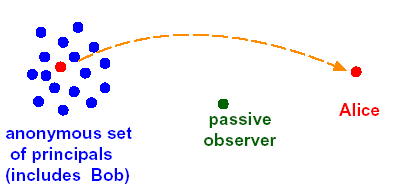
\includegraphics[scale=0.8]{sender-anon.png}
\end{figure}
Receiver anonymity is given, if an observer cannot identify  the receiver of
a message. 
\begin{figure}
    \centering
    \caption[Receiver Anonymity]{Receiver Anonymity\\Image source: \protect\url{http://www.cs.virginia.edu/crab/anonymity.ppt}}
    \label{receiveranon}
    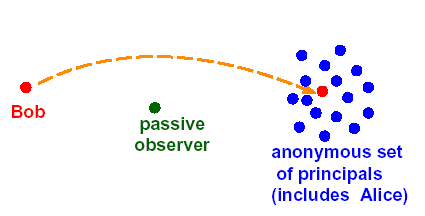
\includegraphics[scale=0.8]{receiver-anon.png}
\end{figure}
If the observer cannot find out whether a given pair of peers
is communicating, Sender-Receiver anonymity is given.
\begin{figure}
    \centering
    \caption[Sender-Receiver Anonymity]{Sender-Receiver Anonymity\\Image source: \protect\url{http://www.cs.virginia.edu/crab/anonymity.ppt}}
    \label{senderreceiveranon}
    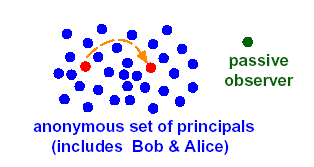
\includegraphics[scale=0.8]{sender-receiver-anon.png}
\end{figure}
The three figures \ref{senderanon}, \ref{receiveranon} and
\ref{senderreceiveranon} visualise the differences.

Although a lot of communication protocols address the challenge
to provide a level of anonymity, this topic has not been covered
by the chat systems. On the other hand, there are various attempts
to allow chat systems to be run in an anonymity network (like I2P), 
though this requires the user, and the peer she wants to talk to,
to install and use the full fledged anonymity network.

The aim of this thesis is to close this gap, to provide a chat system
that provides anonymity, without requiring an additional network stack
to be present.
% -----------------------------------------------------------------------------
\subsection{Confidentiality}
Confidentiality is defined to allow only authorized parties to access
a given set of information. Besides hiding the real content of a conversation,
confidentiality indirectly assists anonymity, because it is not possible to
derive who is talking from the content.

For this reason all messages that are send using the defined chat protocol
have to be treated confidential.
% FIXME: solution:
% We encrypt every message via public-key cryptography\cite{pgp-1},
% so that only the receiver can decrypt and view the message content.
% 
% -----------------------------------------------------------------------------
\subsection{Authenticity}
Authenticity ensures that
\begin{enumerate}
\item the message content has not been modified (integrity is consistent) and that
\item the receiver can verify that the message has been sent by the right person
\end{enumerate}
Both requirements should be supported by the provided chat protocol.
% -----------------------------------------------------------------------------
\subsection{Availability}
Availability in a chat system is important in two directions:
\begin{enumerate}
\item Ensure that receiving messages is possible
\item Ensure that sending messages is possible
\end{enumerate}
Most traditional systems rely on central infrastructure to operate, in which a
single party (like the operator) can disable the service, either for an individual
participant or for the whole network.
Even if a decentralised architecture is given,
no service can be run reliable, if an attacker with infinite resources is assumed.

Thus the requirement for this chat system is to survive the attack of 
a single denial of service attack, which continuing to
be able to send and receive messages.

